\documentclass[11pt, a4paper]{article}
\usepackage{geometry}
\usepackage{tikz}
\usepackage{amsmath}
\usepackage{matlab-prettifier}
\usepackage{inconsolata}
\usepackage[utf8]{inputenc}
\usepackage[T1]{fontenc}
\usepackage{graphicx}
\usepackage{subcaption}
\usepackage{cleveref}



\lstset{
language=Matlab,
style=Matlab-editor,
basicstyle=\ttfamily\footnotesize,
breaklines=true,        % still allows visual wrapping
postbreak=\mbox{\textcolor{gray}{$\hookrightarrow$}\space}, % shows wrap arrow
prebreak={},            % avoids inserting break characters
breakatwhitespace=false,% allows breaking anywhere
columns=flexible,       % better text spacing
keepspaces=true,        % preserve indentation
extendedchars=false,
}

\geometry{a4paper, portrait, margin=3cm}
\begin{document}
	

	



\begin{titlepage}
	\vspace*{\fill}
	\centering
	{\Huge \textbf{Formative Assignment 1: Static MATLAB-Based FEM Modelling} \\}
	{\vspace{2cm}}
	{\large Candidate Number: xxxxx \\}
	{Date: xx/xx/xxxx}

	\vspace{5cm}
	\vspace*{\fill}
		
\end{titlepage}

\normalsize
\tableofcontents

\newpage

\section{Local Element Matrix Functions}
\subsection{Diffusion Operator}

The equation for the local element matrix for the diffusion operator with linear basis functions, is as follows:



\begin{equation}
	k_D
	\begin{bmatrix}
		1 & -1\\
		-1 & 1
	\end{bmatrix}
\end{equation}
	where:
\begin{equation}
	\hspace*{1cm}
	k_D = \frac{D}{2J}
	\hspace*{1cm}
	J = \left|\frac{x_1-x_0}{2}\right| 	
\end{equation}


\subsubsection{Diffusion Matrix Function Code:}


\lstinputlisting{LaplaceElemMatrix.m}

\newpage

\subsubsection{Unit Testing}
\begin{figure}[h]
	\centering
	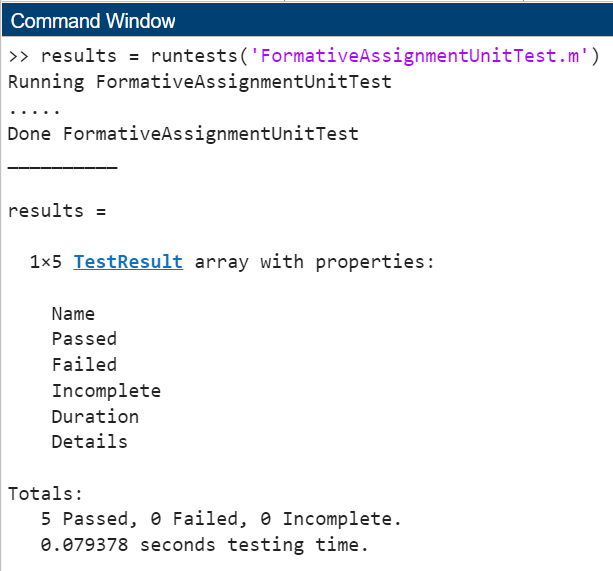
\includegraphics[width=0.65\linewidth]{runtests.png}
	\caption{Result of running unit test with LaplaceElemMatrix.m}
	\label{fig:diff_unit_test}
\end{figure}


\begin{figure}[h]
	\centering
	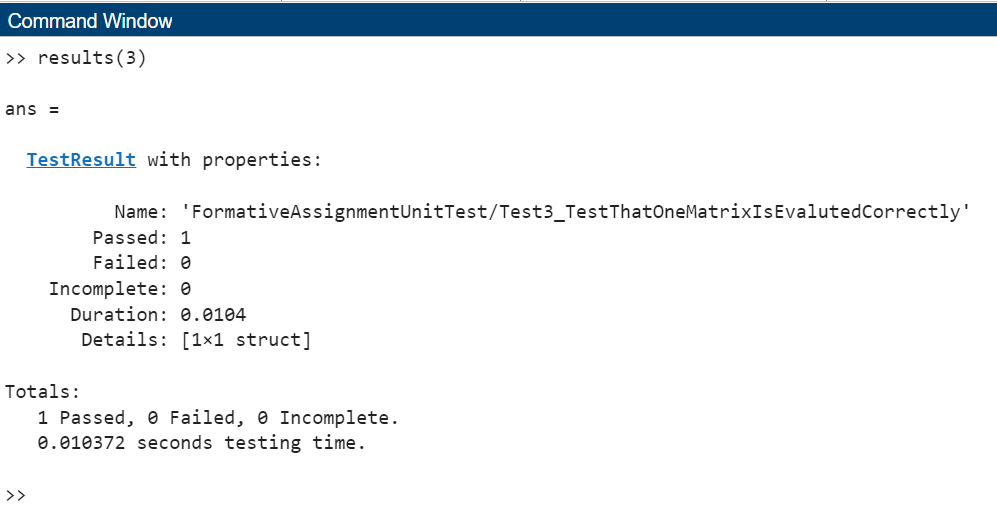
\includegraphics[width=0.65\linewidth]{result3.png}
	\caption{Example test result for Test 3 in unit test}
	\label{fig:diff_test_3}
\end{figure}

\Cref{fig:diff_unit_test,fig:diff_test_3} shows that the local diffusion operator matrix function successfully passed all 5 of the unit tests provided for the task.

\newpage
\subsection{Linear Reaction Operator}

The equation for the local element matrix for the linear reaction operator with linear basis functions is as follows:


\begin{equation}
	k_\lambda
	\begin{bmatrix}
		2 & 1 \\
		1 & 2
	\end{bmatrix}
\end{equation}
Where:
\begin{equation}
	k_\lambda = \frac{J\lambda}{3}
	\hspace{1cm}
	J = \left|\frac{x_1-x_0}{2}\right|
\end{equation}

The unit test function that was provided for the diffusion operator matrix may be replicated and modified for the linear reaction operator. Unit tests 1 and 2 remain valid for the linear reaction operator. Unit tests 3 -5 were updated with the following variables and expected results:
\newline

\begin{center}
	\centering
\begin{tabular}{ |c|c|c|c| }
\hline
Unit Test & $\lambda$ & J & Matrix\\
\hline
 & & & \\[-4mm]
Test 3 & 9 & 0.333 & 
$\begin{bmatrix}
1 & 0.5 \\
0.5 & 1 \\
\end{bmatrix}$\\[3mm]
Test 4 & 12 & 0.5 &
$\begin{bmatrix}
2 & 1\\
1 & 2\\
\end{bmatrix}$\\[3mm]
Test 5 & 12 & 0.0625 &
$\begin{bmatrix}
0.25 & 0.125\\
0.125 & 0.25\\
\end{bmatrix}$\\[3mm]
\hline
\end{tabular}
\end{center}


\subsubsection{Unit Test Code:}

\lstinputlisting{LinearReactionUnitTest.m}

\newpage
\subsubsection{Linear Reaction Matrix Function Code:}

\lstinputlisting{ReactionElemMatrix.m}

\subsubsection{Unit Testing}

\begin{figure}[h]
	\centering
	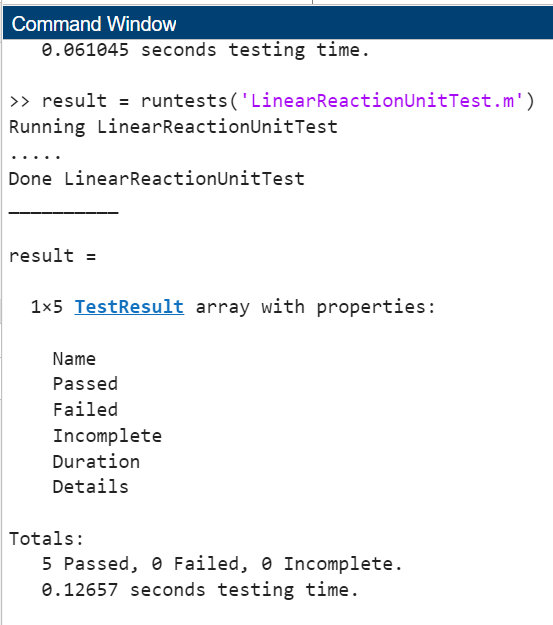
\includegraphics[width=0.7\textwidth]{linearunittest.png}
	\caption{Linear reaction operator unit testing result}
	\label{fig: linear reaction unit test}
\end{figure}

\Cref{fig: linear reaction unit test} shows that the function to create the local element matrix for the linear reaction operator passes all five of the unit tests and, therefore, matches the theory for varying spacial steps. 


\section{Solving Laplace's Equation using FEM}
\section{Verifying FEM Solver for Diffusion-Reaction Equation}
\end{document}